\pagestyle{circuito}
\label{circuito}
%\begin{textblock*}{5.625in}(0pt,0pt)%
%\vspace*{-3.49cm}
%\hspace*{-2.76cm}\includegraphics*[width=175.2mm]{./propagandas/CIRCUITO.pdf}
%\end{textblock*}

\begin{center}
\hspace*{.5cm}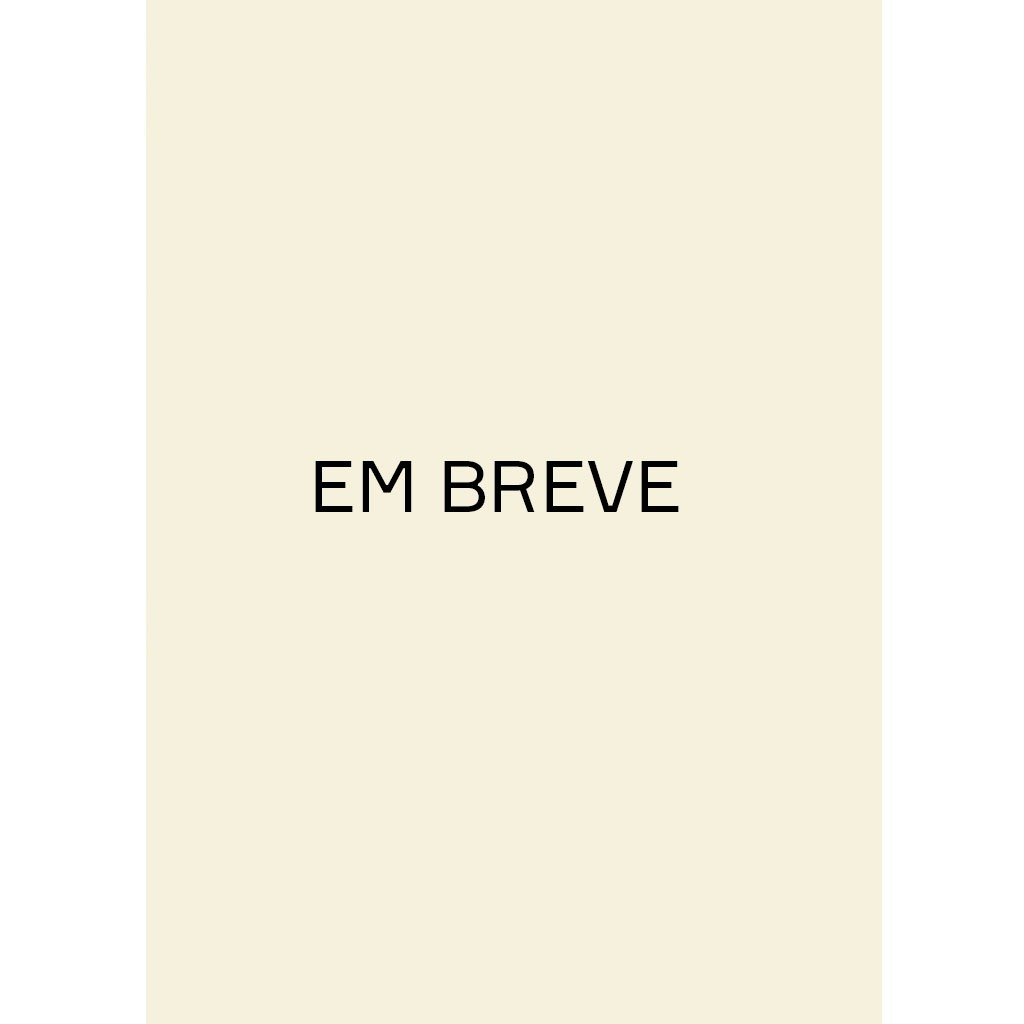
\includegraphics[width=74mm]{./CAPAS/breve.jpeg}
\end{center}
\hspace*{-7cm}\hrulefill\hspace*{-7cm}
\medskip

\noindent{}A publicação de uma segunda edição de \textit{Arte contemporânea brasileira: texturas, dicções, ficções, estratégias} é, sem dúvida, sinal indicativo de que o interesse nas questões trazidas pelo livro permanece em aberto: existiria, ainda, relevância no debate em torno da crítica de arte; seria preciso prestar atenção na presença de uma economia discursiva própria do campo da arte contemporânea --- dinâmicas cuja operatividade desempenharia papéis-chave nas relações que se quer estabelecer com as obras e o circuito, o tecido cultural e as urgências políticas. Amplamente, a presença variada e múltipla da textualidade nos debates compartilhados do campo da arte seria portadora de engajamento, intervenção, provocação e desvio, ao mesmo tempo em que inscreve e estratifica camadas de uma geografia comum da fala e da escrita.

\vfill
\noindent\begin{minipage}[c]{1\linewidth}
{\small\textbf{
\hspace*{-.1cm}Editora: Circuito e Hedra\\
Título: História da arte contemporânea (Vol.\,1)\\
Autor: Ricardo Basbaum (org.)\\ 
ISBN: 978-65-89705-32-1\\
Páginas: Inserir.\\
Formato: 16x23\,cm\\
Preço: R\$ Inserir.\\
}}
\end{minipage}
\pagebreak

\begin{center}
\hspace*{.5cm}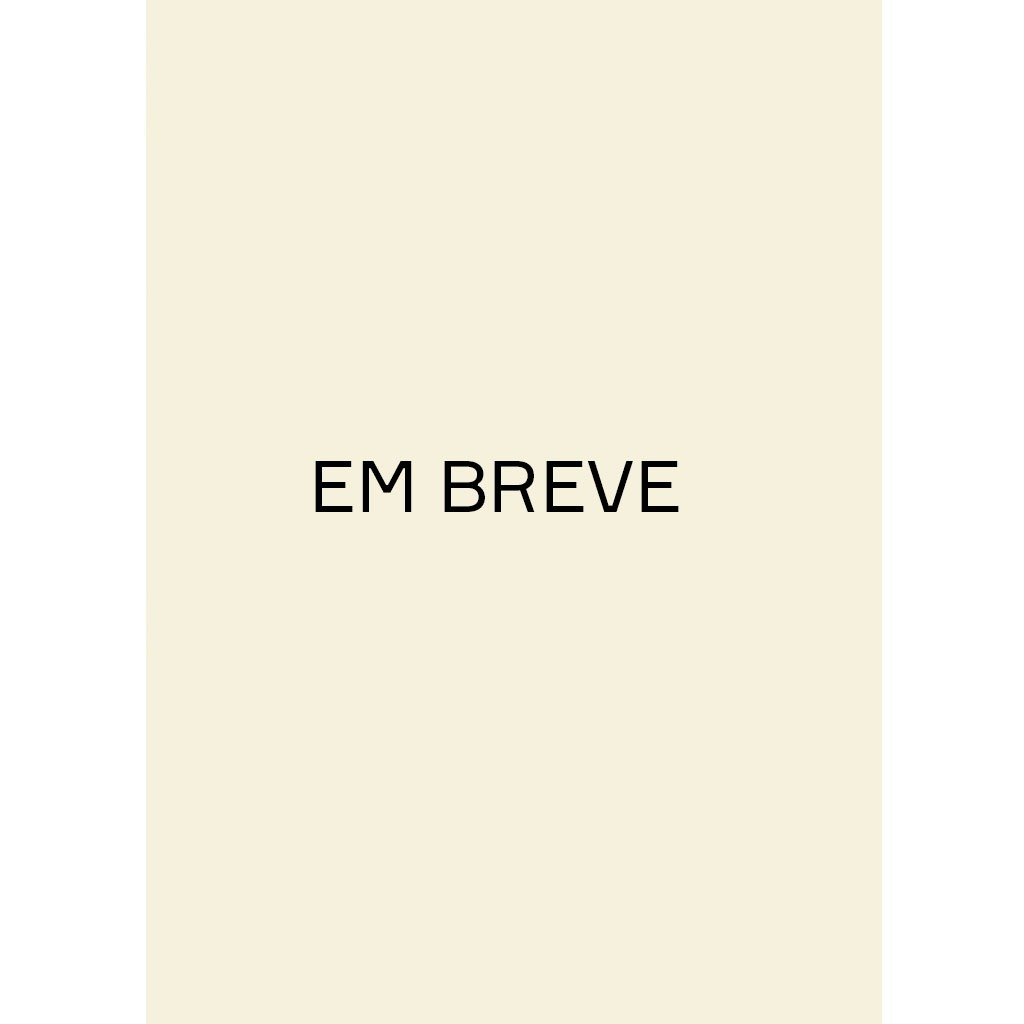
\includegraphics[width=74mm]{./CAPAS/breve.jpeg}
\end{center}
\hspace*{-7cm}\hrulefill\hspace*{-7cm}
\medskip

\noindent{}Tendo como recorte um período especialmente frutífero da arte visual brasileira, esta antologia se apresenta como uma espécie de percurso, no qual espera-se que o saldo final revele algo mais instigante, abundante e reflexivo que uma mera compilação de textos avulsos. São ensaios que dialogam entre si, complementando-se, escritos por artistas, pesquisadores, críticos e curadores de arte em plena atividade. Imaginamos o livro como um mapa, abreviado e conciso, mas indicativo de um território vasto e vibrante: a produção crítico-teórica sobre a arte contemporânea brasileira nas primeiras duas décadas do século XXI. De 2000 a 2020: o arco histórico que abrange parte dos anos FHC e os governos petistas de Lula e Dilma, incluindo as manifestações de 2013 e suas consequências imediatas até o primeiro ano do governo atual --- uma perversa ruptura que exige da arte (e da sociedade como um todo) atenção e ativa militância.

\vfill
\noindent\begin{minipage}[c]{1\linewidth}
{\small\textbf{
\hspace*{-.1cm}Editora: Circuito e Hedra\\
Título: História da arte contemporânea (Vol.\,2)\\
Autor: Renato Rezende (org.)\\ 
ISBN: 978-65-89705-33-8\\
Páginas: Inserir.\\
Formato: 16x23\,cm\\
Preço: R\$ Inserir.\\
}}
\end{minipage}
\pagebreak

\vspace*{1.5cm}
\noindent{}{\nohyphens{\LARGE{Estátua de Glauco}}}
\bigskip

\hfill{}\scalebox{.8}{MARCOS LACERDA}
\bigskip
\bigskip
\bigskip

\begin{multicols}{2}
\noindent{}Por que há ``nada'' onde deveria haver algo? Diferentemente da pergunta
filosófica - porque há algo onde deveria haver nada - esta talvez seja a
indagação que mais se aproxima das questões com que se defronta a arte
brasileira contemporânea. É o susto do vão, do vazio do pensamento, da
subjetividade aberta, ameaçadora e inclassificável. Ali onde deveria
haver "formas sociais" prévias, ou deduzidas, há ``nada'', ou seja, há
estranhos desenhos, pistas falsas, sinuosidades, formas esquivas que se
recusam a classificações e categorizações advindas de quadros de
referências que lhe são radicalmente estranhos. Em suma, abismos.

\textls[-6]{O ambiente com que se depara talvez se aproxime do conhecido mito da
estátua de Glauco de Platão: a imagem divina da estátua, com suas formas
outrora claras e bem delineadas, vai se desfigurando diante da força das
tempestades e do tempo, de tal maneira que nela já não reconhecemos a
forma divina anterior, ela nos parece agora como um animal feroz, de
feições cujo desenho é de uma desordem aterradora, os antigos contornos
legíveis tornando-se deformações assustadoras e enigmáticas. Já não se
sabe bem o que há ali, se a imagem anterior deformada ou se outra imagem
radicalmente distinta da primeira, em suma, já não se sabe se estamos
diante de uma mera alteração de forma, ou de uma mutação ontológica.}

\vspace{\baselineskip}
{\small\fakereceipt{
\noindent{}“Existe um vínculo estreito entre a cultura do neocapitalismo global e movimentações do pensamento baseadas em ideias como dispersão subjetiva,
delírio, fluidez”
}}
\vspace{\baselineskip}

Imaginemos a estátua de Glauco como uma metáfora para se pensar legado
do projeto moderno, tanto na feição iluminista, romântica e simbolista,
quanto na modernista. Estaríamos vivendo um momento de mutação
ontológica sem precedentes, com o advento de fenômenos como o do
"pós-modernismo", do "pós-colonialismo", do pós-humanismo, do "Império"
e das "sociedades de redes"? Ou seria uma alteração, astuta e
sorrateira, da lógica de predomínio do Capital, entendido quase sempre
como o sujeito adequado à estrutura para se pensar a modernidade,
associada agora à dessublimação repressiva, ao imperativo do gozo, à
noções do senso comum difuso como as de fluidez, desterritorização,
pluralização subjetiva e diversidade?

Diante da emersão de uma pluralidade de formações subjetivas na
contemporaneidade, provindas de um processo de desrecalque que
acompanha, por sua vez, processos históricos e políticos de ampla
envergadura como a descolonização, mas também o capitalismo global
desterritorializado e o multiculturalista liberal, ainda é possível
sintetizar tal pluralidade em noções como as de ``humanidade do homem",
devedoras de projetos políticos cuja centralidade reside no Ocidente
Europeu? Não deveríamos ficar mais atentos à ``pluriversidade
transmoderna'' que pode forjar ``teorizações bárbaras'' não
necessariamente imanentes à modernidade, neste sentido com um conjunto
de discurso muito distante do discurso filosófico da modernidade?

O livro apresenta alguns desses temas. A sua estrutura se organiza entre
dois polos: crítica às tentativas de restauração do projeto moderno, com
suas loas à melancolia e à resignação, segundo a análise dos autores, e
tomada de posição por um ``salto ao abismo do contemporâneo''. O
desenrolar das reflexões e dos capítulos sugere que teríamos um processo
de passagem a fazer, quase como um rito, num primeiro momento de
desconstrução, para usar um termo da moda, e num segundo de possível
construção.

Para que a passagem se realize, assim, é necessário uma espécie de
expiação. E ela teria que se dar através da crítica, com o
reconhecimento do mérito, de movimentações profundas do processo de
modernização das artes no Brasil, como a Semana de 22 centrada em São
Paulo, o concretismo, também paulistano e a arquitetura de Brasília,
marcos decisórios do Brasil moderno. A estes elementos, poderíamos unir
a ausência/presença do pensamento crítico e do marxismo heterodoxo da
USP. Tudo sintetizado e tendo como pano de fundo o racionalismo
ocidental, o colonialismo europeu e à crítica à ``humanidade do homem''
como essência inegociável do humanismo.

O livro tem como sua fundamentação teórica principal o conceito de
trauma, base de um dos principais campos de conhecimento da modernidade,
a psicanálise, de extração freudiana. É por ele que vai se desdobrando,
fio a fio, às vezes de maneira mais condensada, com articulações que
seguem muito bem a dinâmica da clareza de base acadêmica, outras de modo
mais solto, deixando a própria sensibilidade imagética das obras se
expressar nas palavras que, neste caso, são como formas concretas e não
meios para representar mensagens, ou mesmo meio de representação, como
bem nos ensinou o concretismo brasileiro.

Os primeiros parágrafos que abrem a introdução são belos e enigmáticos,
tem algo de alegórico, o significado das palavras se confunde com um
quadro repartido de imagens de pensamento estilhaçadas e condensam de
forma instigante séculos de história, arte e política. Explicitam o
sentido do contemporâneo, enovelado na problemática do trauma e
envolvido de forma densa em acontecimentos religiosos, estéticos e
políticos. Paulo e o caminho de Damasco. Caravaggio. As finalidades sem
fim do Ocidente. O irrepresentável, aquilo que foge a qualquer forma de
figuração possível. O que não pode ser simbolizado, o que escapa à
linguagem e se expressa como desvio, movimento sem forma, abismo.

\textls[-4]{As experimentações mais cruéis da modernidade do século XX, como a bomba
atômica e os campos de concentração, seriam realidades cuja
monstruosidade interrompe a racionalidade, a beleza da limpidez da
forma, a concatenação de ideias como articulação entre imagem,
pensamento e intuição. Ficamos com a opacidade, a face desfeita, o corpo
despido de vitalidade existencial, o tremor diante do terrificante. Mas
a arte é terrível, precisa seguir. E tem dado respostas. O livro
apresenta duas: a negação do enfrentamento do trauma, pensada também
como negação ao abandono do projeto da modernidade; o seu enfrentamento,
com a coragem do salto ao abismo e, aí sim, a possível realização do
contemporâneo.}

\textls[-6]{Tal perspectiva parece ecoar, a nosso ver, a ambivalência da modernidade
por excelência, entre a constatação crítica da dominação estrutural e
sistêmica, embora com tons de resignação melancólica segundo os autores,
e a consciência da possiblidade de emancipação, com a sensibilidade
aguda para as linhas de fuga que podem permitir o salto. As melhores
interpretações e críticas à modernidade, diga se de passagem, souberam
mostrar a sua ambivalência trágica, sem aderir necessariamente a nenhum
dos polos, seja o que aparentemente paralisa diante do abismo, ou o que,
também aparentemente, dá o salto.}

Mas é fundamental ainda acrescentarmos mais uma alternativa que, a nosso
ver, perpassa e, ao mesmo tempo, desafia o sentido do contraponto entre
moderno e contemporâneo, tal qual tratado no texto: a adesão ao efeito
narcotizante da espetacularização do pensamento, na estética e na
política em tempos de cultura do capitalismo como imperativo do gozo e
dessublimação repressiva. Existe um vínculo estreito entre a cultura do
neocapitalismo global e movimentações do pensamento baseadas em ideias
como dispersão subjetiva, delírio, fluidez, estímulo à vivência da
intensidade do instante, relativismo sarcástico e irracionalismo
pulsional.

\bigskip
\noindent{}\textcolor{gray}{\footnotesize\slsc{\textls[-15]{Texto adaptado do posfácio do livro “Trauma — Arte contemporânea”.}}}
\end{multicols}

\pagebreak
\pagestyle{circuitocat}
\begin{multicols}{2}
\begin{enumerate}
\raggedright\nohyphens{
\item A grande marcha, \textbf{Ewerton Martins Ribeiro }
\item A loucura branca, \textbf{Jaime Rocha}
\item A outra morte de Alberto Caeiro, \textbf{Afonso Henriques Neto}
\item A Dialética do gosto, \textbf{Marco Scheinder}
\item Adoecer, \textbf{Hélia Correia}
\item Almas selvagens, \textbf{André Gardel}
\item Até ano que vem em Jerusalém, \textbf{Maria da Conceição Caleiro}
\item Cadernos de artista, \textbf{Moisés Alves}
\item Cérebro-Ocidente/Cérebro"-Brasil, \textbf{Roberto Corrêa dos Santos}
\item Nove tiros em Chef Lidu, \textbf{Paula Bajer Fernandes}
\item Comunidades sem fim, \textbf{João Camillo Penna e Ângela Maria Dias (orgs.)}
\item Coletivos, \textbf{Renato Rezende e Felipe Scovino (orgs.)}
\item DJs, \textbf{Fred Coelho e Joca Vidal (orgs.)}
\item Dezembro, \textbf{Ana Tereza Salek}
\item Os tigres cravaram as garras no horizonte, \textbf{Augusto Guimaraens Cavalcanti}
\item No contemporâneo: arte e escritura expandidas, \textbf{Roberto Corrêa dos Santos; Renato Rezende}
\item Truques de autor, \textbf{Heleno Bernardi}
\item Clínica de artista I, \textbf{Roberto Corrêa dos Santos}
\item Clínica de artista II, \textbf{Roberto Corrêa dos Santos}
\item Vertigens, \textbf{Fernanda de Mello Gentil}
\item Nós somos uma correspondência, \textbf{Fernanda de Mello Gentil}
\item Amarração, \textbf{Renato Rezende}
\item Conversas com curadores e críticos de arte, \textbf{Renato Rezende e Guilherme Bueno (orgs.)}
\item Experiência e arte contemporânea,  \textbf{Renato Rezende e Ana Kiffer (orgs.)}
\item Romance, \textbf{Caio Meira}
\item Auréola, \textbf{Renato Rezende}
\item Cosmocrunch, \textbf{Maria Dolores Wanderley}
\item Preces para a amiga submersa, \textbf{Lucia Castello Branco}
\item Pequena coleção de grandes horrores, \textbf{Luiz Brás}
\item Nós, o outro, o distante na arte brasileira contemporânea, \textbf{Marisa Flórido Cesar}
\item Lira dos sentidos, \textbf{Carlos Henrique Costa}
\item Rasga-mortalha: poemas dos outros, \textbf{W. B. Lemos}
\item Os nomes, \textbf{Rogério Luz}
\item N’Ágorainda, \textbf{Naila Rachid}
\item O ser-se, \textbf{Júnia Azevedo}
\item A reflexão atuante, \textbf{Sergio Cohn}
\item Intervenções críticas, \textbf{Josefina Ludmer}
\item O homem mais portátil do mundo, \textbf{Arturo Carrera}
\item O capitão Nemo e eu, \textbf{Alfredo Prior}
\item Notas, disparos, sublinhados, \textbf{María Moreno}
\item Naxos, \textbf{Elsa Cross}
\item Diário em progresso, \textbf{Alex Frechette}
\item Em caso de emergência pare o tempo, \textbf{Gab Marcondes}
\item 1,68 x 1,81, \textbf{Maria André Leite}
\item Do tudo e do todo, \textbf{Cláudio Oliveira}
\item S.O.S. Poesia, \textbf{Renato Rezende; Dirk Vollenbroich}
\item O olho do lince, \textbf{Guilherme Zarvos}
\item Diário para descolorir, \textbf{Alex Frechette}
\item A pequena voz do mundo, \textbf{Diana Bellessi}
\item Amazônia \& Co., \textbf{Rafael Cippolini}
\item Fala, poesia, \textbf{Tamara Kamenszain}
\item Suturas. Um breviário, \textbf{Daniel Link}
\item Repetir, \textbf{Katia Maciel}
\item Coreografia (Orelhas contemporâneas), \textbf{André Parente}
\item Amor: verso: reverso (Orelhas contemporâneas), \textbf{Luiz Sérgio de Oliveira}
\item Saudades de um punhal (Orelhas contemporâneas), \textbf{Leila Danziger}
\item Gravidade (Orelhas contemporâneas), \textbf{Katia Maciel}
\item Artexperiência contemporânea (Orelhas contemporâneas), \textbf{Renato Rezende}
\item Práticas contemporâneas do mover-se, \textbf{Michelle Sommer}
\item Levantem lentamente o lençol, \textbf{Bia Albernaz}
\item Escritos sobre fotografia contemporânea brasileira, \textbf{Antonio Fatorelli, Victa de Carvalho e Leandro Pimentel (orgs.)}
\item Doctypes, \textbf{Alex Hamburger}
\item Quarenta e quatro, \textbf{Mauricio Cardozo}
\item Ninfas e Mariposas, \textbf{Leonardo Toledo}
\item Lab Criativo / Creative Lab, \textbf{Paul Heritage, Batman Zavarese (orgs.)}
\item Quase-poesia, \textbf{Jerson Lima Silva}
\item Música Chama, \textbf{Pedro Sá Moraes; Eduardo Guerreiro B. Losso}
\item Viventes de Saturno, \textbf{Carlos Frederico Manes}
\item Esperando a hora da Stella, \textbf{Maria Dolores Wanderley}
\item Falar o que seja é inútil – ou sobre desconsiderações, \textbf{Carlos Alberto Gianotti}
\item Lótus molotov, \textbf{Leonardo Toledo}
\item Outras margens, \textbf{Sergio Cohn}
\item Formas híbridas, \textbf{Rafael Gutiérrez}
\item Fornicar e matar e outros ensaios, \textbf{Laura Klein}
\item Cores cobras pincéis cães, \textbf{Eduardo Stupía}
\item Lasca de breu, \textbf{Guilherme Delgado}
\item O tropo tropicalista, \textbf{João Camillo Penna}
\item Leituras furadas, \textbf{Luis Felipe Fabre}
\item Escrever sobre escrever poesia, \textbf{Eduardo Milán}
\item A liberação da mosca, \textbf{Luigi Amara}
\item Mudança, \textbf{Verónica Gerber Bicecci}
\item Onde late um cachorro doido, \textbf{Moisés Alves}
\item Daniel Acosta
\item Éter, \textbf{António Cabrita}
\item Noturno Europeu, \textbf{Rui Nunes}
\item Café irlandês, \textbf{Barbosa Lagos}
\item Voo, \textbf{Ana Paula Simonaci}
\item Fim do Infante, \textbf{Marina Marcondes Machado}
\item 2013, memórias e resistências, \textbf{Camila Jourdan}
\item Escrito e dirigido por Moisés Alves, \textbf{Moisés Alves}
\item Coisas que fiz e ninguém notou mas que mudaram tudo, \textbf{Moisés Alves}
\item A cena lenta, \textbf{Cláudio Oliveira}
\item Copa pra quem? Olimpíadas pra quem?, \textbf{Alex Frechette}
\item O fantasma de um nome (poesia, imaginário, vida), \textbf{Jorge Monteleone}
\item Peso Morto, \textbf{João Felipe Gremski}
\item Romance de asilo, \textbf{André Monteiro}
\item Quem apaga a luz sou eu, \textbf{Magda Romano}
\item As artes do cover, \textbf{Henrique Saidel}
\item Frestas, \textbf{André Gardel}
\item O antes é o depois, \textbf{Guidi Vieira}
\item Humano, \textbf{Pedro Poeta}
}
\end{enumerate}
\end{multicols}

\pagebreak
